\documentclass[10pt]{article}

% ====================================================
% PACKAGES
% ====================================================
\usepackage[margin=0.75in, headheight=13.6pt]{geometry}
\usepackage[T1]{fontenc}
\usepackage{lmodern}
\usepackage{microtype}
\usepackage{setspace}
\usepackage{tcolorbox}
\usepackage{amsmath, amssymb, mathtools}
\usepackage{siunitx}

\usepackage{graphicx}
\usepackage{float}
\usepackage{subcaption}
\usepackage{wrapfig}

\usepackage{enumitem}
\usepackage{booktabs}
\usepackage{array}
\usepackage{multirow}

\usepackage{xcolor}
\usepackage{hyperref}

\usepackage{fancyhdr}
\usepackage{lastpage}
\usepackage{indentfirst}
\usepackage[justification=centering]{caption}

\pagestyle{fancy}
\fancyhf{}
\lhead{\Assignment\ |\ \course}
\rhead{\Name\ |\ \today}
\cfoot{Page \thepage\ of~\pageref{LastPage}}

\hypersetup{
    colorlinks,
    linkcolor={red!50!black},
    citecolor={blue!50!black},
    urlcolor={blue!80!black}
}

\newcommand{\Name}{Arael Anaya}
\newcommand{\Assignment}{Project Update}
\newcommand{\course}{Advanced Dynamics (MEGN505)}

% Highlighted note box (e.g., for the meeting date/time)
\newtcolorbox{noteBox}{
    colback=blue!3!white,
    colframe=blue!40!black,
    boxrule=0.6pt,
    arc=2pt,
    left=6pt, right=6pt, top=4pt, bottom=4pt
}

\setlength{\parskip}{0.25em}
\setlength{\parindent}{0pt}

\begin{document}

% ====================================================
% TITLE
% ====================================================
\begin{center}
    {\Large \textbf{Project Update: Dynamics and Stability of the Spring-Loaded Inverted Pendulum (SLIP) Model}}\\[2pt]
    \Name
\end{center}
\vspace{-4pt}

% ====================================================
% (a) MOTIVATION
% ====================================================
\subsection*{(a) System and Motivation}
For my final project I am modeling the spring-loaded inverted pendulum
(SLIP) model of a hopping/running robot -- the reduced-order model that
underlies essentially all legged-robot dynamics. Despite its simplicity (a
point mass bouncing on a massless spring leg), the SLIP model captures the
center-of-mass dynamics of running in both animals and machines
remarkably well, making it simple enough to analyze rigorously with the
tools from this course while still producing rich, interesting behavior.
It also builds naturally on the elastic pendulum system studied in class,
since the stance phase is essentially an inverted spring pendulum.

% ====================================================
% (b) METHODS
% ====================================================
\subsection*{(b) Modeling Methods}
The SLIP model is a hybrid dynamical system, shown schematically in
Figure~\ref{fig:progress}: during stance the body behaves as a
spring-loaded pendulum, while during flight it is simply a projectile. I
am deriving the equations of motion for each phase using the Lagrangian
formulation in polar coordinates $(r,\theta)$ for the stance phase,
together with the switching conditions at touchdown and liftoff that
connect the two phases. To assess stability of the hopping gait itself
(rather than just a single equilibrium), I will use an apex return map --
a Poincar\'e map in which a periodic hopping gait appears as a fixed point
whose stability can be evaluated numerically \cite{blickhan1989}. The
model will be implemented in Python using event-based numerical
integration, with a parameter study over spring stiffness and touchdown
angle.

% ====================================================
% (c) PROGRESS
% ====================================================
\subsection*{(c) Progress to Date}
TODO: Summarize the progress made so far -- e.g., which equations of
motion have been derived, whether the touchdown/liftoff switching
conditions are implemented, whether the Python simulation runs, and any
preliminary results (e.g., a first stance-phase trajectory or return-map
point).

\begin{figure}[H]
    \centering
    \vspace{-4pt}
    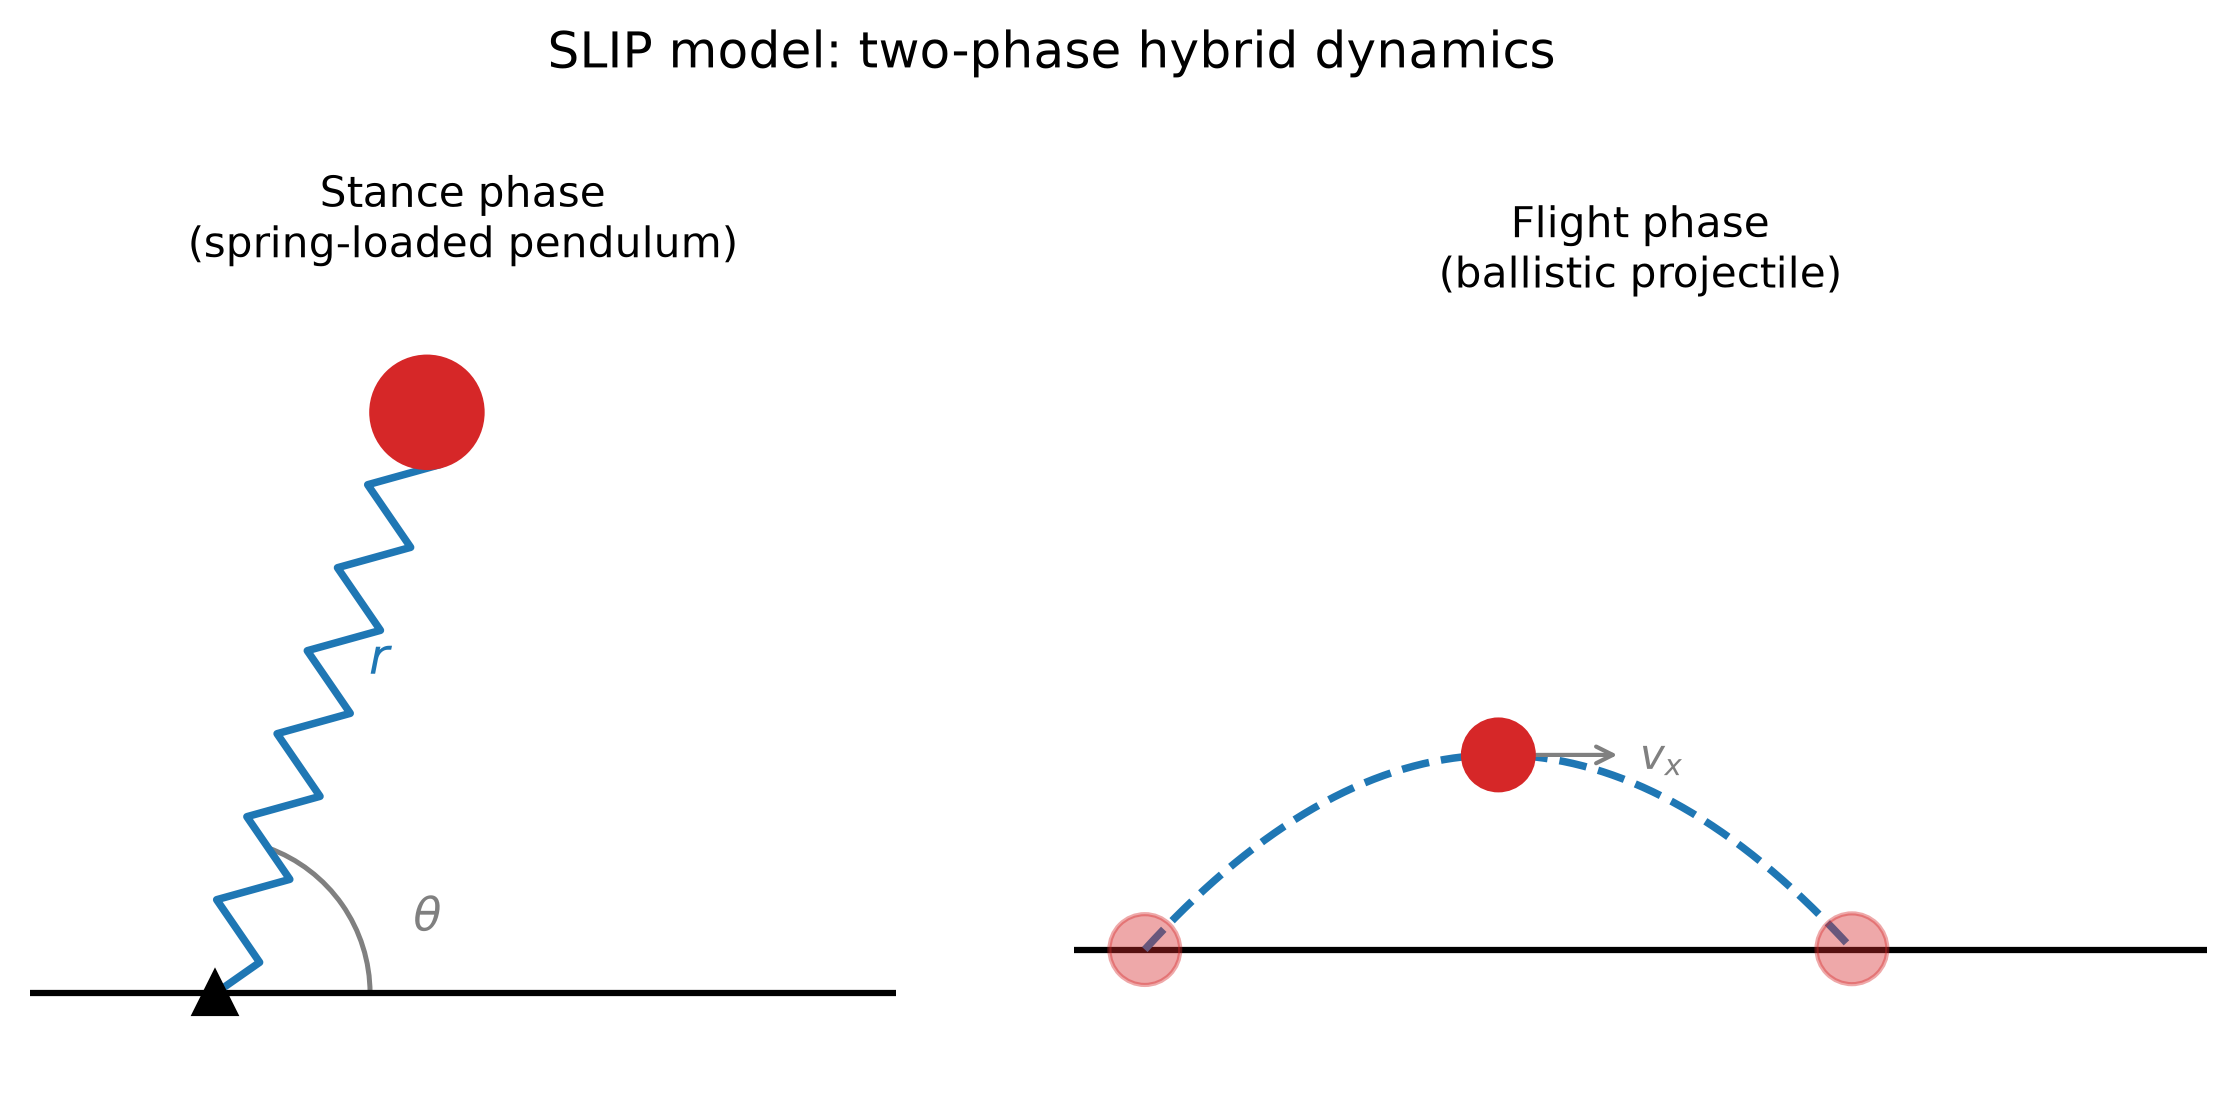
\includegraphics[width=0.55\linewidth]{Figures/progress_figure.png}
    \vspace{-6pt}
    \caption{\footnotesize Schematic of the SLIP model's two-phase hybrid
    dynamics: stance (spring-loaded pendulum in polar coordinates
    $r,\theta$) and flight (ballistic projectile).}
    \label{fig:progress}
\end{figure}
\vspace{-8pt}

% ====================================================
% MEETING NOTE
% ====================================================
\begin{noteBox}
\small\textbf{Scheduled update meeting:} TODO -- day, date, and time.
\end{noteBox}

% ====================================================
% REFERENCES
% ====================================================
\footnotesize
\begin{thebibliography}{9}
\setlength{\itemsep}{0pt}
\bibitem{blickhan1989}
R.~Blickhan, ``The spring-mass model for running and hopping,''
\textit{Journal of Biomechanics}, vol.~22, no.~11--12, pp.~1217--1227,
1989.
\end{thebibliography}

\end{document}
